%% BioMed_Central_Tex_Template_v1.06
%%                                      %
%  bmc_article.tex            ver: 1.06 %
%                                       %

%%IMPORTANT: do not delete the first line of this template
%%It must be present to enable the BMC Submission system to
%%recognise this template!!

%%%%%%%%%%%%%%%%%%%%%%%%%%%%%%%%%%%%%%%%%
%%                                     %%
%%  LaTeX template for BioMed Central  %%
%%     journal article submissions     %%
%%                                     %%
%%          <8 June 2012>              %%
%%                                     %%
%%                                     %%
%%%%%%%%%%%%%%%%%%%%%%%%%%%%%%%%%%%%%%%%%


%%%%%%%%%%%%%%%%%%%%%%%%%%%%%%%%%%%%%%%%%%%%%%%%%%%%%%%%%%%%%%%%%%%%%
%%                                                                 %%
%% For instructions on how to fill out this Tex template           %%
%% document please refer to Readme.html and the instructions for   %%
%% authors page on the biomed central website                      %%
%% http://www.biomedcentral.com/info/authors/                      %%
%%                                                                 %%
%% Please do not use \input{...} to include other tex files.       %%
%% Submit your LaTeX manuscript as one .tex document.              %%
%%                                                                 %%
%% All additional figures and files should be attached             %%
%% separately and not embedded in the \TeX\ document itself.       %%
%%                                                                 %%
%% BioMed Central currently use the MikTex distribution of         %%
%% TeX for Windows) of TeX and LaTeX.  This is available from      %%
%% http://www.miktex.org                                           %%
%%                                                                 %%
%%%%%%%%%%%%%%%%%%%%%%%%%%%%%%%%%%%%%%%%%%%%%%%%%%%%%%%%%%%%%%%%%%%%%

%%% additional documentclass options:
%  [doublespacing]
%  [linenumbers]   - put the line numbers on margins

%%% loading packages, author definitions

\documentclass[twocolumn]{bmcart}% uncomment this for twocolumn layout and comment line below
%\documentclass{bmcart}

%%% Load packages
\usepackage{amsthm,amsmath}
\RequirePackage{natbib}
%\RequirePackage[authoryear]{natbib}% uncomment this for author-year bibliography
\RequirePackage{hyperref}
\usepackage[utf8]{inputenc} %unicode support
%\usepackage[applemac]{inputenc} %applemac support if unicode package fails
%\usepackage[latin1]{inputenc} %UNIX support if unicode package fails


%%%%%%%%%%%%%%%%%%%%%%%%%%%%%%%%%%%%%%%%%%%%%%%%%
%%                                             %%
%%  If you wish to display your graphics for   %%
%%  your own use using includegraphic or       %%
%%  includegraphics, then comment out the      %%
%%  following two lines of code.               %%
%%  NB: These line *must* be included when     %%
%%  submitting to BMC.                         %%
%%  All figure files must be submitted as      %%
%%  separate graphics through the BMC          %%
%%  submission process, not included in the    %%
%%  submitted article.                         %%
%%                                             %%
%%%%%%%%%%%%%%%%%%%%%%%%%%%%%%%%%%%%%%%%%%%%%%%%%

%% -- switch these when needed
%\RequirePackage{graphicx}  % added by mct
\def\includegraphic{}
\def\includegraphics{}



%%% Put your definitions there:
\startlocaldefs
\def\app{OVAS}
\newcommand{\triplesub}[2]{\noindent\textsl{#1}\\#2\\}  % think of it as a \subsubsubsection{}

%\newcommand\changes
\newcounter{changeCount}
\newcommand{\changes}[1]{
	\stepcounter{changeCount}
	{\tiny\bf\color{violet}\arabic{changeCount}}
	{\color{red} #1}
}



\endlocaldefs


%%% Begin ...
\begin{document}

%%% Start of article front matter
\begin{frontmatter}

\begin{fmbox}
\dochead{Research}

%%%%%%%%%%%%%%%%%%%%%%%%%%%%%%%%%%%%%%%%%%%%%%
%%                                          %%
%% Enter the title of your article here     %%
%%                                          %%
%%%%%%%%%%%%%%%%%%%%%%%%%%%%%%%%%%%%%%%%%%%%%%

\title{\app{}: an open-source variant analysis suite}

%%%%%%%%%%%%%%%%%%%%%%%%%%%%%%%%%%%%%%%%%%%%%%
%%                                          %%
%% Enter the authors here                   %%
%%                                          %%
%% Specify information, if available,       %%
%% in the form:                             %%
%%   <key>={<id1>,<id2>}                    %%
%%   <key>=                                 %%
%% Comment or delete the keys which are     %%
%% not used. Repeat \author command as much %%
%% as required.                             %%
%%                                          %%
%%%%%%%%%%%%%%%%%%%%%%%%%%%%%%%%%%%%%%%%%%%%%%

\author[
   addressref={aff1},                   % id's of addresses, e.g. {aff1,aff2}
   email={},   							% email address
   noteref={n1}
]{\inits{}\fnm{Monika} \snm{Mozere}}
\author[
   addressref={aff1},
   email={m.tekman@ucl.ac.uk},
   noteref={n1}
]{\inits{}\fnm{Mehmet} \snm{Tekman}}
\author[
   addressref={aff2},
   email={}
]{\inits{A}\fnm{Jameela} \snm{Kari}}
\author[
   addressref={aff1},
   email={}
]{\inits{}\fnm{Detlef} \snm{Bockenhauer}}
\author[
   addressref={aff1},
      corref={aff1},
   email={r.kleta@ucl.ac.uk}
]{\inits{}\fnm{Robert} \snm{Kleta}}
\author[
   addressref={aff1},
   email={h.stanescu@ucl.ac.uk}
]{\inits{}\fnm{Horia} \snm{Stanescu}}

%%%%%%%%%%%%%%%%%%%%%%%%%%%%%%%%%%%%%%%%%%%%%%
%%                                          %%
%% Enter the authors' addresses here        %%
%%                                          %%
%% Repeat \address commands as much as      %%
%% required.                                %%
%%                                          %%
%%%%%%%%%%%%%%%%%%%%%%%%%%%%%%%%%%%%%%%%%%%%%%
 
\address[id=aff1]{%                                                   % unique id
  \orgname{Division of Medicine, University College London}, % university, etc
  \city{London}                              % city
  \postcode{NW3 2PF,}                          % post or zip code
  \cny{UK}                                    % country
}
\address[id=aff2]{%
  \orgname{Pediatric Nephrology Center of Excellence and Pediatric Department,
Faculty of Medicine, King Abdulaziz University},
  \city{Jeddah},
  \cny{Kingdom of Saudi Arabia}
}

%%%%%%%%%%%%%%%%%%%%%%%%%%%%%%%%%%%%%%%%%%%%%%
%%                                          %%
%% Enter short notes here                   %%
%%                                          %%
%% Short notes will be after addresses      %%
%% on first page.                           %%
%%                                          %%
%%%%%%%%%%%%%%%%%%%%%%%%%%%%%%%%%%%%%%%%%%%%%%

\begin{artnotes}
%\note{Sample of title note}     % note to the article
\note[id=n1]{Equal contributor} % note, connected to author
\end{artnotes}

%\end{fmbox}% comment this for two column layout

%%%%%%%%%%%%%%%%%%%%%%%%%%%%%%%%%%%%%%%%%%%%%%
%%                                          %%
%% The Abstract begins here                 %%
%%                                          %%
%% Please refer to the Instructions for     %%
%% authors on http://www.biomedcentral.com  %%
%% and include the section headings         %%
%% accordingly for your article type.       %%
%%                                          %%
%%%%%%%%%%%%%%%%%%%%%%%%%%%%%%%%%%%%%%%%%%%%%%

\begin{abstractbox}

\begin{abstract} % abstract


\parttitle{Background}\
The advent of modern high-throughput genetics continually broadens the gap between the rising volume of sequencing data, and the tools required to process them. The need to pinpoint a small subset of functionally important variants has now shifted towards identifying the critical differences between normal variants and disease-causing ones. The ever-increasing reliance on cloud-based services for sequence analysis and the non-transparent methods they utilize has prompted the need for more in-situ services that can provide a safer and more accessible environment to process patient data, especially in circumstances where continuous internet usage is limited.

\parttitle{Results}\
To address these issues, we herein propose our standalone Open-source Variant Analysis Sequencing \emph{(\app{})} pipeline; consisting of three key stages of processing that pertain to the separate modes of annotation, filtering, and interpretation. Core annotation performs variant-mapping to gene-isoforms at the exon/intron level, append functional data pertaining the type of variant mutation, and determine hetero/homozygosity. Up to 12 filtering modules can be used in sequence ranging from single quality control to multi-file penetrance model specifics such as X-linked recessive or mosaicism. Depending on the type of interpretation required, additional annotation is performed to identify organ specificity through gene expression and protein domains. In the course of this paper we analysed an autosomal recessive case study. \app{} made effective use of the filtering modules to recapitulate the results of the study by identifying the prescribed compound-heterozygous disease pattern from exome-capture sequence input samples.

\parttitle{Conclusion}
\app{} is an offline open-source modular-driven analysis environment, designed to annotate and extract useful variants from Variant Call Format (VCF) files, and process them under an inheritance context through a top-down filtering schema of swappable modules, run entirely off a live bootable medium and accessed locally through a web-browser.

%\parttitle{Supplementary information} Supplementary data is available from \textit{BMC-Bioinformatics} online.\\
\end{abstract}

%%%%%%%%%%%%%%%%%%%%%%%%%%%%%%%%%%%%%%%%%%%%%%
%%                                          %%
%% The keywords begin here                  %%
%%                                          %%
%% Put each keyword in separate \kwd{}.     %%
%%                                          %%
%%%%%%%%%%%%%%%%%%%%%%%%%%%%%%%%%%%%%%%%%%%%%%

\begin{keyword}
\kwd{open source}
\kwd{variant analysis}
\kwd{disease model}
\kwd{mosaic}
\kwd{bootable}
\kwd{live environment}
\end{keyword}

% MSC classifications codes, if any
%\begin{keyword}[class=AMS]
%\kwd[Primary ]{}
%\kwd{}
%\kwd[; secondary ]{}
%\end{keyword}

\end{abstractbox}
%
\end{fmbox}% uncomment this for twcolumn layout

\end{frontmatter}

%%%%%%%%%%%%%%%%%%%%%%%%%%%%%%%%%%%%%%%%%%%%%%
%%                                          %%
%% The Main Body begins here                %%
%%                                          %%
%% Please refer to the instructions for     %%
%% authors on:                              %%
%% http://www.biomedcentral.com/info/authors%%
%% and include the section headings         %%
%% accordingly for your article type.       %%
%%                                          %%
%% See the Results and Discussion section   %%
%% for details on how to create sub-sections%%
%%                                          %%
%% use \cite{...} to cite references        %%
%%  \cite{koon} and                         %%
%%  \cite{oreg,khar,zvai,xjon,schn,pond}    %%
%%  \nocite{smith,marg,hunn,advi,koha,mouse}%%
%%                                          %%
%%%%%%%%%%%%%%%%%%%%%%%%%%%%%%%%%%%%%%%%%%%%%%

%%%%%%%%%%%%%%%%%%%%%%%%% start of article main body

%%%%%%%%%%%%%%%%
%% Background %%
%%
\section*{Background}
The technological evolution of sequencing platforms has progressed rapidly since the completion of the Human Genome project via Sanger sequencing methods \cite{lander2001initial,sanger1977dna}. Modern high-throughput sequencing (HTS) approaches post-Sanger era have superseded this standard, allowing for a greater number of variants to be sequenced across the whole genome by employing powerful mass fragmentation/amplification approaches upon a target sequence \cite{lengauer2007bioinformatics,bockenhauer2012genetic}.

%pabinger2014survey

The raw sequence FASTQ reads produced by these HTS platforms are aligned to a specific version of the NCBI reference sequence and collated into a Binary Alignment Map (BAM) where variants of interest can then be individually "called" to form a Variant Call Format (VCF) file of novel or known variants conforming to a specific variant database (dbSNP) \cite{li2009sequence,danecek2011variant}.

BAM and VCF data are orthogonally related, with the former storing horizontal stretches of FASTA sequence reads aligned unevenly on top of one another forming "pile ups", and the latter taking vertical cross-sections of these pileups at specific loci to form a variant call.

The VCF specification was designed for the 1000 Genomes project to produce a robust format that could house the many samples often sequenced under the same batch, but has since been adopted by projects such as UK10K, dbSNP, NHLBI Exome Project, amongst others. The format is flexible with annotations, where additional fields can be outlined in the header and adhered to in the body of the data. Each line of the VCF body describes a single variant; physical position paired with a reference allele (as ascribed by a reference genome consistent across the entire VCF file) and alternate alleles that appear within samples. Major and minor alleles are specific only to the sample population but their frequencies can be pre-computed and appended to a variant line as additional information to then be utilized in small population analyses such as inheritance modelling \cite{danecek2011variant}.

Variant analysis suites all work under the same principle; filtering variants under a user-specified set of criteria against the various variant annotations present in the VCF in order to produce a subset informative to the phenotype. \changes{Conservative filtering measures will produce a smaller set with the drawback of missing key causative variants, and more optimistic filtering measures will produce too many false positives}. The effectiveness of an analysis rests primarily upon the accuracy of the variant annotations which can attribute to as much as 15\% of false negatives \cite{warden2014detailed}, as well as the frequency of false negatives that are discarded due to overly-stringent quality filtering. A common approach to addressing both issues is through learning algorithms that can be trained to favour individual variants over others with the caveat of producing results via 'black-box' methods that may create some disparity between the user and their data \cite{pabinger2014survey}.

A more transparent approach is to expand the scope of the filtering beyond the variant / gene-level and explore variants under a larger trait-penetrance context.% outlined in Figure~\ref{fig:inheritance}.

Mendelian traits conform to the four classical modes on inheritance of autosomal / X-linked, dominant / recessive penetrance. Dominant disorders result from the inheritance of a single mutant allele which is manifested in each subsequent generation with a 50\% chance of likelihood in offspring from a single affected parent. Recessive traits require the inheritance of two mutant alleles on opposing strands in order to block any functioning copies of the causative gene. Parents are typically carriers with affected offspring. These disorders are at times a result of consanguineous marriages, where a single mutant allele manifests on both alleles due to the multiple paths of descent it can undertake \cite{kari2014consanguinity}. In the case of X-linked recessive inheritance, males with a single mutant copy are hemizygous and must express the phenotype. % as shown in Figure~\ref{fig:inheritancex}.

For non-Mendelian disorders, we also consider the special case of \textit{mosaicism}; where de novo mutations produce two or more populations of cells that result in segregated sets of genotypes within the same individual. Mosaic genotypes can be revealed stochastically by measuring alternate allele frequencies against expected values \cite{biesecker2013genomic}.

Here we outline our Open-source Variant Analysis Suite (\app{}) that makes use of these inheritance modelling scenarios with the aim to vastly reduce the number of false positives.

\section*{Implementation}
The core ideology behind \app{} was to preserve the VCF specification at each step of the analysis, and this is catered to extensively within the pipeline where each module inputs and outputs VCF file(s) in order to facilitate the chaining of subsequent pipeline modules downstream. This allows for full analysis transparency, where results can be extracted at any stage of an ongoing analysis.

Module ordering is flexible in this regard, with the exception of the primary annotation modules which are required to run prior to any filtering in order to produce an effective analysis of the variants. Pre-existing gene and function annotations within input data are ignored unless generated by a previous run of the \app{} pipeline, supplanting foreign annotations with the pipeline's own if required. This is to ensure unambiguous results stemming from external annotations using unknown sources that may result in erroneous output variants.

\changes{\app{} annotates variants using data pulled from trusted public domain databases such as RefGene, dbSNP, UniProt, and many others through the UCSC Genome Browser's MySQL back-end portal \cite{karolchik2003ucsc}}. The explicitly open nature of pipeline also prompts a predilection towards open-source or scripted languages and frameworks, which further serve to uphold the confidence between the end-user and their data.

\changes{Core pipeline functionality is managed through back-end shell scripts which serve to chain subsequent pipeline modules as shown in Figure~\ref{fig1}. The modular-centric design and development enables each pipeline module to be run as a standalone script without the need for an overarching framework. It also allows for the pipeline to be initiated manually for the more commandline-oriented users, where input VCF files can be placed into a new folder on the desktop along with a pedigree file and an appropriate configuration file (see manual in Supplemental Data), and executed via the starting script. 

However, \app{} was designed to cater towards all users, and is accessed primarily through a graphical user-interface within a web browser which facilitates in the VCF file placement and configuration process through file selection dialogues and configurable forms to generate run profiles, as well a means to manage and view ongoing analyses as shown in Figure~\ref{fig2}.

\app{} is split into three separable parts, with each component encapsulated by the next; the processing back-end, the web-interface front-end, and the live operating system. Instructions to acquire and set up each as distinct items are provided in the software repository, but \app{} is bundled principally as an all-encompassing standalone bootable ISO image that can be deployed onto a DVD or USB.}


\subsection{Pipeline Overview}

\changes{\app{} is split into five main stages of processing followed by a generated report detailing the findings of the analysis.\\

\triplesub{\bf Pre-processing}{All VCF files immediately undergo initial preparation upon file submission from the web interface, where a background shell script renames the files to better emulate their pedigree counterparts, and asserts that all variants are in correct order following a chromosome:position sorting scheme.}

\triplesub{\bf Core Annotation}{
The annotation stages of the pipeline then affix the variants with the relevant metadata to aid in the filtering process against user-specified criterion throughout the rest of the pipeline.

First, a gene context is appended to the variants specific to a level of detail preferred by the user. This includes, but is not limited to; exons, introns, (donor/acceptor) splice sites, (5'/3') UTR, and (default 500bp) upstream/downstream promoters. Wholly intergenic regions are discarded by default, which often results in a vast majority of initial variants being filtered out (approximately 90\% for whole-genome sequence data).

Ensuing functional changes and the resulting mutation types (synonymous, missense, nonsense, etc) are also annotated to the variant by performing cDNA lookups of the variant against reference genome FASTA data and determining the subsequent changes at the codon and amino-acid level for all sense and anti-sense gene transcripts, as well as frameshifts caused by indels.

The VCF specification generally denotes a single variant per line and OVAS vehemently upholds this policy when a variant bisects multiple gene transcripts. This is notably different from UCSC's Variant Annotator, which despite taking in VCF input, does not preserve the format and reports multiple bisecting sites upon adjacent lines. For a given variant, OVAS ensures that each gene context and correlating functional change are stored in-line as separate associative arrays that are indexed to the same gene transcript.

Finally, heterozygosity and homozygosity are assigned to the variant based on nucleotide base count alone, addressing a confidence issue in the zygosity assignment provided by pre-processed variants.
}

\triplesub{\bf Filtering}{
Once fully annotated, variants are then subject to the conventional filtration modules that act upon the standard positional and INFO fields provided by VCF data against regions/thresholds set by the user. Specifically; \textit{Physical Location Filter}, \textit{Novel Variation Filter}, \textit{Read Depth Filter}, and \textit{Call Quality Filter}.

OVAS provides a \textit{Mutation Type Filter} which acts upon the functional annotations provided by OVAS to keep/discard any variation of missense, nonsense, and synonymous mutations. It also provides an \textit{Alternate Allele Frequency} module which screens for rarity by comparing alternate allele frequencies against the reference genome via dbSNP (version 147).

Variants are also filtered over multiple VCF files, with the \textit{Same Variant Filter} discarding variants not shared across all cases, and the \textit{Same Gene Filter} discarding those that do not reside within the same gene context shared across all cases. Both modules are used extensively in the inheritance filters.
}}

\triplesub{\bf Inheritance Filtering}{
This section performs trait penetrance modelling for differently affected individuals following sibling-sibling, and sibling-parent relations. For all detected parent-offspring trios, variants undergo context-based filtering depending on the penetrance-model specified:\\

	\triplesub{Autosomal Dominant}{The phenotype is caused by a single mutant autosomal allele, and affected individuals must have affected parents, mapping any \{HOM,HET\}$\mapsto$\{HET,HOM\} under complete penetrance. Under a \textit{de novo} context all common affected variants are filtered against unaffected controls, otherwise variant commonality is kept within sibling groups.}

	\triplesub{Autosomal Recessive}{
The phenotype is caused by a loss of function stemming from both copies of an autosomal gene, at times from the result of consanguineous breeding. Two paths of transmission are considered from parent$\mapsto$offspring depending on whether the affected offspring variant is compound-heterozygous (C-HET) or homozygous (HOM). Under the assumption that parents are carriers:\\
	\begin{enumerate}
\item{\bf HOM}{, Both parents transmit a single HET variant which manifests as a single HOM variant in the offspring, i.e. \{HET/HET\}$\mapsto$HOM.}
\item{\bf C-HET}{, Parents are carriers for different HET variants across a common gene, which compound in offspring as multiple HET variants within said gene. If HET1 and HET2 are distinct variants within the same gene from different parents, then this can be represented under a gene context as \{HET1/HET2\} $\mapsto$ \{HET1+HET2\} mapping to produce a C-HET gene.}
	\end{enumerate}
	\vspace{5pt}
Siblings are then filtered for common variants existing within affecteds siblings only, discarding those that are homozygous in unaffected controls.

	\triplesub{X-linked Dominant}{As with autosomal dominant but with the mutant allele on the X-chromosome.}
	
	\triplesub{X-linked Recessive}{As with autosomal recessive but with mutations occurring on the X-chromosome. Males with a single mutant copy are hemizygous and are treated as homozygous, exempting them from compound heterozygosity checking.}
	
	\triplesub{Mosaicism}{Mosaic inheritance is treated as a special case, where allele frequencies are pre-calculated for each variant and then filtered against user-set thresholds conforming to expected mosaic frequency ranges (typically between 10-35\%).}
}

\changes{\triplesub{Extended annotation}{The last processing stage of pipeline constitutes a small set of potentially causative variants that successfully passed through the main filtering stages and require finer annotation and analysis that was too costly to perform for all variants at the start. Here, gene transcripts are assigned RefSeq IDs to better distinguish them against external sources(\textit{Isoform Context}), variants falling within known protein domains provided by UniProt are further functionally annotated (\textit{Protein Context}), and tissue-specific data from the Encode GNF Atlas2 database are used to filter for/against genes falling within user-specified gene expression thresholds (\textit{Gene Expression}).}

\triplesub{Web Report}{All remaining variants across all output VCF files are then consolidated into an interactive HTML table which summarizes variants under sortable and filterable columns of chromosome, position, rsID, gene, gene context, cDNA and protein change, functional change, and heterozygous/homozygous occurrence in cases and controls (see Figure~\ref{fig3}). This provides a good overview of potentially causative variants, especially in recessive disease models where compound-heterozygosity can occur.
}}
}

%%%%%%%%
\section*{Results}

Here we describe the case study results for two autosomal recessive and one X-linked dominant disease models.

\subsection*{First Case Study}

Three families presented with hyperinsulinemic hypoglycemia and congenital polycystic kidney disease (HIPKD), a rare newly discovered disorder following an autosomal recessive model. Whole-genome linkage analysis in conjunction with haplotype reconstruction hinted towards a compound-heterozygous disease pattern in all cases within a significant locus on chromosome 16 \cite{cabezas2017polycystic}.

Exome-capture sequencing of all cases revealed a promoter mutation paired with either a missense or splice site mutation. To recapitulate the results of this study within \app{}, all four cases were inserted into the pipeline of which two were siblings, permitting the use of variant-level filtering. Pedigree overviews as well as runtime settings conforming to those in the supplemental material of the preceding paper are displayed in the analysis interface (Figure~\ref{fig2}).

%Of the 9 input VCF files, 4 were affected cases of which 2 were siblings. The remaining VCFs were controls consisting of 4 (2 pairs) of unaffected parents and 1 was unaffected sibling, permitting the use of variant-level filtering.

Each VCF file comprised of approximately 250,000 variants (SNPs and InDels) and were profiled against a gene map at the first annotation step (\textit{Adding Genes}) comprised of exons, donor/acceptor essential splice sites (5bp), and upstream/downstream promoter regions (500bp). Reference genes as well as their isoforms were also retained in the analysis.

The prior linkage analysis \cite{cabezas2017polycystic} hinted at a small region of interest (16p13.3-16p13.2 spanning 2.93 Mbp) populated by 11 genes and 40 isoforms, and applying this locus via the \textit{Physical Location Filter} resulted in 99.9\% of variants being filtered out.

%To address the effectiveness of the \app{} without the bias implicit by the results of the genetic linkage analysis, two types of run configurations were explored; the first that applied the linkage-derived locus immediately following the mandatory \textit{Core Annotation} stage, and the second that applied the locus as the last step in the pipeline.

The \textit{Core Annotation} stage accounted for the vast majority ($ > 80\% $) of the exome-sequenced variants being filtered out in both scenarios, intersecting variants against the gene map (declared previously) in order to remove those that were entirely intergenic or (non-regulatory) intronic. This resulted in approximately 34,700 annotated variants ready for the subsequent filtering modules.

The subsequent application of the the \textit{Physical Linkage Filter} reduced the number of variants to less than 25 in each case file (Figure~\ref{fig4}). The \textit{Call Quality Filter} with a threshold of $>20$ was applied in accordance to the filtering criterion in the original study, resulting in a 25.7\% reduction. The rarity of the phenotype prompted a search for variants not very prevalent in the population, thus the \textit{Alternate Allele Frequency Filter} (AAF) was applied with a threshold of $< 1\%$, leaving no more than 10 variants in each case file. The \textit{Autosomal Recessive Inheritance Filter} (AR) then performed identical variant level matching between the two affected siblings, screened against homozygous mutations, and followed compound-heterozygous checking upon all files to produce an overlapping AR gene list. 

Truncating under this provided just 4 variants in each file (5 unique in total), and applying the final \textit{Mutation Type Filter} to remove any synonymous mutations resulted in just 2 variants in each file (3 unique in total) that successfully produced a characteristic compound-heterozygous AR inheritance pattern in \textit{PMM2}; \textit{c.-167G}$>$\textit{T} promoter variant in all, \textit{c.422G}$>$\textit{A} missense mutation in three of the cases, and a \textit{c.255+1G}$>$\textit{A} splice site mutation present in one case (Figure~\ref{fig3}).

%The second scenario (Figure~\ref{fig4} (bottom)) performed the annotation as with the first scenario, but this time only reduced an average of 15.9\% of variants in the \textit{Call Quality Filter} step to approximately 37,000 variants. The \textit{Alternate Allele Frequency Filter} reduced this to under 21,000 rare variants, and the \textit{Autosomal Recessive Inheritance Filter} further trimmed this to approximately 10,000 variants, whereupon applying the final \textit{Physical Linkage Filter}, outlined less than 9 output variants in each case.

\changes{
\subsection*{Second Case Study}
A  single  family  displaying  a  phenotype  under  an  X-linked dominant inheritance model. Whole-exome sequencing was performed upon 8 individuals (7 affected, 1 unaffected) with almost 290,000  variants in each VCF file. 

As before, the first annotation step filtered out the majority of variants, with an 89.3\% reduction due to variants being wholly intergenic/intronic. Significant linkage  analysis  outlined  a  narrow  region  of  interest upon chromosome X, which coupled with the \textit{Physical Location Filter} reduced the initial set to just 351 variants (Figure S1 (top)). A cascade of filters targeting novel  non-synonymous  mutations  under  an  X-linked dominant scenario (common across affecteds) resulted in a single causative missense variant.


\subsection*{Third Case Study}

Four siblings were presented from a consanguineous marriage with a nephrotic syndrome segregating in an autosomal recessive fashion. Exome-sequencing was
performed on each sibling with an initial targeted set of approximately 70,000 variants. Core annotation accounted for a 65.9\% reduction in total variants, and a missense/nonsense \textit{Mutation Type Filter} reduced the initial set to under 11,000 variants (Figure S2 (bottom)). Due to the rarity of phenotype, the AAF module was utilized to filter for any variants with a frequency less than 0.01 within dbSNP (version 142), vastly reducing the number to a cluster of 878 variants.

Applying the autosomal recessive inheritance module with same variant filtering resulted in just 15 variants common across affecteds only, of which 2 were
homozygous in different genes. Additional gene expression annotation was prioritized; with one variant conforming to a standard house-keeping gene expression
profile, and the other being the more likely disease-causing variant due to it displaying a strong organ specific expression.
}



%% DISCUSSION
\section*{Discussion}

Depending upon the total input variants as well as the number and ordering of modules used, an average initial analysis using any number of modules (excluding alternate allele filtering) for VCF files containing 300,000 variants each, will attribute a total of 2 minutes per VCF.

There are several limiting steps however, with the largest bottleneck occurring at initial gene annotation stage, which must prime all input variants for downstream filtering through the use of a gene (or exon) map that is dependent upon user parameters. Gene maps for a variety of user parameters already exist as static files in the live environment, but not all use-cases are covered and a new gene map must be generated for custom configurations which can take up to 1 hour to retrieve depending on internet speed and proximity to the closest UCSC MySQL mirror.

In the case of general gene map use-cases, the \textit{Adding Genes} annotation step still requires 200 times more processing time than most other modules, and was the sole reason that all annotation modules were re-written in C++ to benefit from a significant performance increase that reduced the module's processing time from an initial time of 10 minutes to under 3 minutes (Table~\ref{table:results}). 

The rest of the annotation modules are comparatively much faster, with the functional annotations experiencing mild latency related to disk read speeds when performing repeated byte-offset lookup upon FASTA files. The initial sorting of the variants upon file upload is valuable in this regard due to the higher tendency of adjacent variants to share the same disk cluster and reap paging benefits.

Across subsequent pipeline runs, processing is not repeated for the same data; each module checks whether an input VCF file has already been processed by the current pipeline configuration, and repeatedly iterates through the module ordering until the last processed input set is reached where it can resume processing.

\subsection{Case Performance}

The case analysis completed its run in 10.2 minutes, with subsequent re-runs upon pre-annotated data completing in under 1 minute. 

It is not without doubt that the order of filtering modules is important to the analysis, with the \textit{Physical Location Filter} decreasing the runtime of subsequent modules. However this decrease is sub-linear in complexity as shown in Table~\ref{table:results}, which displays average individual timings for each module against moderately populated VCF files, showing that runtimes are comparable with the case analysis with the exception of the AAF module.

The AAF module created an noticeable lag of an average of 7.27 seconds per file in our study. This is owing to the module being subject to some delay in loading pre-computed dbSNP allele frequencies into memory, and due to memory and processing constraints, it must incur this cost for each new chromosome encountered which can create considerable latency in the earlier (larger) chromosomes. The analysis escaped this penalty somewhat by only having to load a single relatively small chromosome into memory.


%The second scenario produced the almost the exact same output variants as the first scenario with the exception of case 22 which produced one extra variant in the analysis, despite using the exact same filters as the first with a single ordering modification. The cause of the discrepancy between these results is due to the method in which the \textit{Autosomal Recessive Inheritance Filter} processes compound-heterozygosity, whereby the module casts a conservative net over all genes that are intersected at least twice by variants. Given the number of overlapping regions (gene, gene isoforms, promoters, UTRs, and Splice Sites) that can be bisected by any variant, the number of potential compound-heterozygous genes can increase substantially with the pool of available variants.

\subsection{Transparency and Deployment}

The portability of \app{} grants a significant advantage over present-day web-based pipelines by keeping all analyses securely \textit{in situ}, which is greatly beneficial to regions of the world without consistent or active internet in addition to researchers handling personal or private data. 

\changes{The need for accessible offline tools is most present in Africa, where bioinformatical infrastructure and resources are limited, often requiring international collaborations to advance the study of their own data \cite{h3africa2014enabling}.

Cloud-based pipelines provide processing power without incurring the hardware cost, but the progression of large whole-genome sequencing data coupled with restricted internet speeds hinder the uptake of these services somewhat as slow transfer speeds ultimately dictate service viability; a factor that is further confounded by the net neutrality debate \cite{netneutrality}.} Cloud-based analyses also require input data to be uploaded to an external server in order to perform processing, and data ownership after upload is not always retained especially in the case where the work was performed within the cloud \cite{reed2010information}. Further, many cloud-services employ non-transparent proprietary methods to reduce the number of false-positives and false-negatives. A common approach is to make use of an internal database or learning algorithm that favours some variants over others based on previous analyses (or a similar training set) \cite{pabinger2014survey}, resulting in informative variants produced by unquantifiable "black-box" means, creating disparity between the end-user and their analysis.

Transparent filtering methods are likelier to instil greater confidence in the data with the added benefit of customization to better tailor a filter to an analysis in the case of open-source implementations, as with the case of \app{}.


\changes{
\app{} is bundled within a lightweight Arch Linux environment that contains the pipeline and the web server, static files, and a minimal desktop environment. 
This is in direct contrast to the more familiar virtualization container platforms such as Docker or Vagrant which provide snapshots of an existing OS, and then must then be run off a virtualization layer that uses more hardware resources during input/output operations than if the OS was run natively \cite{virtualcomparison}. Where virtualization strategies permit wider avenues of deployment, \app{} is specialized to be deployed on bootable mediums and is heavily optimized in this respect in terms of storage and runtime efficiencies which allow it to be run more readily upon more limited hardware by culling any resource-consuming middleware.
}

%difference of philosophy

\changes{Initial development considered the use of pre-existing implicit convention frameworks such as \textit{Snakemake} \cite{koster2012snakemake}, but a predilection towards coding-flexibility and processing efficiency (especially with respect to extensive use of standard system input/ouput streams) meant that a more unix-driven pipeline framework was required. \app{} uses an over-arching shell-script framework that adheres to good-practice dependency and re-entrancy concepts \cite{leipzigreview}, by managing file dependencies between adjacent modules and by permitting resumeable workflows such that a VCF file will not undergo the same annotation module twice if it has already been processed under the same inputs.}


\changes{
\subsection{Comparison to Other Bioinformatic Utilities}

\citeauthor{pabinger2014survey} surveys 205 bioinformatic tools, of which 12 are open-source workflows comparable to \app{} live environment, and 13 are standalone open-source pipelines similar to \app{}'s web-server and shell pipeline combination.

% UCSC Variant Annotator
A further 32 variant annotation utilities are also compared; 10 which can take VCF files as input but only 4 of which output annotated VCF files (ANNOVAR, AnnTools, NGS-SNP, SeattleSeq,). Other annotators either focus more on upstream genomic formats (FASTA / BAM) or they produce report summaries of the variants; most likely to escape the potential pitfall of the same  variant intersecting multiple sites. \app{} overcomes this limitation by enclosing multiple sites and their related annotations as sideways associative arrays, and treating each site as a single entity when performing filtering later on in the pipeline. 

In



\app{} also appears to be the only variant annotator that covers a full range of variant types (SNP / Indel / CNV), appends functional annotations on downstream changes to protein structure, and can be used both via the commandline and web interface (see Table S1).

A total of 25 free and open-source (FOSS) pipelines and workflows are also compared; 5 pipelines able to handle VCF files and 2 able to perform annotation (GATK, HugeSeq). HugeSeq uses ANNOVAR for annotation, 
GATK hosts a wide range of VCF annotation modules, but are focused mostly on quality control and allele metrics, but does not perform functional annotations. 


is commandline-oriented but does plan to host a cloud-server that provides a user-interface




\subsubsection{Variant Annotation}
Pabinger compares 32 variant annotators, of which only 9 take VCF files as input and which a staggering 4 produce VCF output (AnnTools, AnnoVar, NGS-SNP, SeattleSeq Annotation).

Chasm, SNVbox, and F-SNP perform functional annotations but none of them apply the annotations to the VCFs.

AnnTools and Annovar cover a full range of variants (SNP / Indel/ CNV) whereas the other two handle only either SNPs or SNPs with indels. In terms of access, AnnTools Annovar and NGS-SNP are strictly commandline, whereas SeattleSeq is strictly Web-based; none provide access to both. 


\subsubsection{Pipelines}

13 pipelines, of which 5 handle VCF (Bcbio-nextgen, GATK, HugeSeq, Ngs-backbone, RTG). All handle Illumina with some Solid data. All have commandlines and are not cloud based. All cater linux, with 2 (Bcbio,RTG) catering to all mac and windows too, of which BcBio has a GUI. Only two perform annotation (GATK, HugeSeq) with HugeSeq using Annovar for annotation.

\subsubsection{Workflows}

12 workflows, with coverage for illumina and solid, and Linux requirements. All GUI, 5 which offer CLI access (KNIME, LONI, Moa, Taverna, Yabi).
How many accessible to bioinformaticians and not programmers?
  - Programmers: 
        Ergatis
        Genboree - but cannot be deployed locally.
        GeneProf
        Taverna - IDE heavy
  - BioInfs: 
        Galaxy
        GenePattern
        Kepler
        KNIME (VCF oriented)
        LONI
  - Other:
        Moa used mostly for alignment
        Yavi is not accesible.
        
        

Over 200 bioinformatic pipelines are in existence, with the majority being online. The most highly cited is the Galaxy web server.



}


%% CONCLUSIONS

\section*{Conclusions}

The self-contained environment provided by \app{} allows researchers to tailor all aspects of their analysis and retain control of their data sets at any phase of processing by means of the transparent open-source modules that comprise the pipeline. 

The live environment, paired with the web front-end, provides the additional advantage of abstracting the end-user from the underlying platform specifics by streamlining the input and configuration process, as well as logging active progress descriptions for the current stage of processing, and lastly providing a malleable final report upon all remaining variants discovered complete with dynamic filtering capabilities. The entirety of all uploaded variants are processed first at the gene annotation stage, placing significant strain at the initial stage of the pipeline that is only managed through the use of employing C++ binaries to overcome the performance bottleneck that would otherwise exist with Python/Bash scripts.

The annotation step is crucial, especially for whole-genome sequence data where the vast majority of the variants would be deemed wholly intergenic and would be filtered out as uninformative to the analysis. More common exome-sequencing data typically observe less of a reduction at a much faster processing rate due to the smaller number of total variants, but at the impediment of missing regulatory elements due to lack of coverage. Modules downstream of the annotation stage run trivially, and due to the pipeline's resume feature which prevents \app{} from processing the same data twice, many subsequent analyses with different module configurations can be run in quick succession after the initial annotation step is complete.

\app{} is future-secure due to the inclusion of the background scripts that generated the static data being packaged with the live environment. Updates to the human genome reference, variant databases, and FASTA sequences can be retrieved on demand for platforms with active internet connections. Changes will preserve across successive boots for non-volatile storage mediums such as USB sticks, ideal in deployment scenarios with infrequent or absent internet access.


%%%%%%%%%%%%%%%%%%%%%%%%%%%%%%%%%%%%%%%%%%%%%%
%%                                          %%
%% Backmatter begins here                   %%
%%                                          %%
%%%%%%%%%%%%%%%%%%%%%%%%%%%%%%%%%%%%%%%%%%%%%%

\begin{backmatter}

\section*{Availability of Data and Materials}
\app{} was developed using C++, Python, Bash, Php, Javascript, and HTML under a Linux OS. It is free software licensed under GPLv3, with the source code and live ISO binary image freely accessible for download at \url{https://bitbucket.org/momo13/ovas-pipeline.git}. The data that support the results of this study have been sanitized against subsequential incidental findings as outlined by ACMG recommendations \cite{kalia2016recommendations}, and are available upon request. The \app{} pipeline can either be directly installed locally on a pre-existing Linux OS, or it can be accessed in-situ by booting the live image.


\section*{List of Abbreviations}
\textbf{UTR}:  Untranslateable Region, \textbf{cDNA}: Complementary DNA,\\
\textbf{HET}: Heterozygous, \textbf{HOM}: Homozygous,\\
\textbf{C-HET}: Compound-Heterozygous, \textbf{SNP}: Single Nucleotide Polymorphism,\\
\textbf{InDel}: Insertion-Deletion, \textbf{LOD}: Logarithm of the Odds,\\
\textbf{HTS}: High-Throughput Sequencing, \textbf{VCF}: Variant Call Format,\\
\textbf{BAM}: Binary Alignment Map, \textbf{OS}: Operating System,\\
\textbf{CNV} : Copy Number Variant, \textbf{FOSS} : Free and Open Source,\\
\textbf{HIPKD}: Hyperinsulinemic hypoglycemia and polycystic kidney disease,\\




% https://bmcbioinformatics.biomedcentral.com/submission-guidelines/preparing-your-manuscript/software-article
\section*{Ethics approval and consent to participate}
Ethics approval and consent was provided by the ethics committee of Royal Free Hampstead NHS Trust (committee's reference number R\&D ID 7727).

\section*{Competing interests}
The authors declare that they have no competing interests.

\section*{Author's contributions}
MM designed and implemented the filtering, extended annotation, and disease model-specific scenario Python modules. MT wrote the core annotation C++ utilities, and reworked the pipeline into the live ISO bootable environment. The pipeline workflow was structured by MM and implemented by MT. The study of genomic data sets given by JAK and DB prompted the conception of the pipeline. HS was instrumental to the development process by providing method evaluation, feature requests, and overall technical supervision. HS and RK provided quality control assessment and agreed to be accountable for all aspects of the work in ensuring that questions related to the accuracy or integrity of any part of the work are appropriately investigated and resolved. All authors considered, discussed, read, and approved the final manuscript.



\section*{Funding}
This work was supported by St. Peter's Trust for Kidney, Bladder and Prostate Research, the David and Elaine Potter Charitable Foundation, Kids Kidney Research, Garfield Weston Foundation, Kidney Research UK, the Lowe Syndrome Trust, the Mitchell Charitable Trust, and the European Union, FP7 (grant agreement 2012-305608 ``European Consortium for High-Throughput Research in Rare Kidney Diseases (EURenOmics)''). Part of this work was also supported by the Deanship of Scientific Research, King Abdulaziz University, Jeddah, grant number 432/003/d to JAK, DB and RK.


%%%%%%%%%%%%%%%%%%%%%%%%%%%%%%%%%%%%%%%%%%%%%%%%%%%%%%%%%%%%%
%%                  The Bibliography                       %%
%%                                                         %%
%%  Bmc_mathpys.bst  will be used to                       %%
%%  create a .BBL file for submission.                     %%
%%  After submission of the .TEX file,                     %%
%%  you will be prompted to submit your .BBL file.         %%
%%                                                         %%
%%                                                         %%
%%  Note that the displayed Bibliography will not          %%
%%  necessarily be rendered by Latex exactly as specified  %%
%%  in the online Instructions for Authors.                %%
%%                                                         %%
%%%%%%%%%%%%%%%%%%%%%%%%%%%%%%%%%%%%%%%%%%%%%%%%%%%%%%%%%%%%%

% if your bibliography is in bibtex format, use those commands:
\bibliographystyle{spbasic} % Style BST file (bmc-mathphys, vancouver, spbasic).
\bibliography{bibliography}      % Bibliography file (usually '*.bib' )
% for author-year bibliography (bmc-mathphys or spbasic)
% a) write to bib file (bmc-mathphys only)
% @settings{label, options="nameyear"}
% b) uncomment next line
%\nocite{label}


%%%%%%%%%%%%%%%%%%%%%%%%%%%%%%%%%%%
%%                               %%
%% Figures                       %%
%%                               %%
%% NB: this is for captions and  %%
%% Titles. All graphics must be  %%
%% submitted separately and NOT  %%
%% included in the Tex document  %%
%%                               %%
%%%%%%%%%%%%%%%%%%%%%%%%%%%%%%%%%%%

%%
%% Do not use \listoffigures as most will included as separate files

%\section*{Figures}
%
\begin{figure}[h!]
  %\centerline{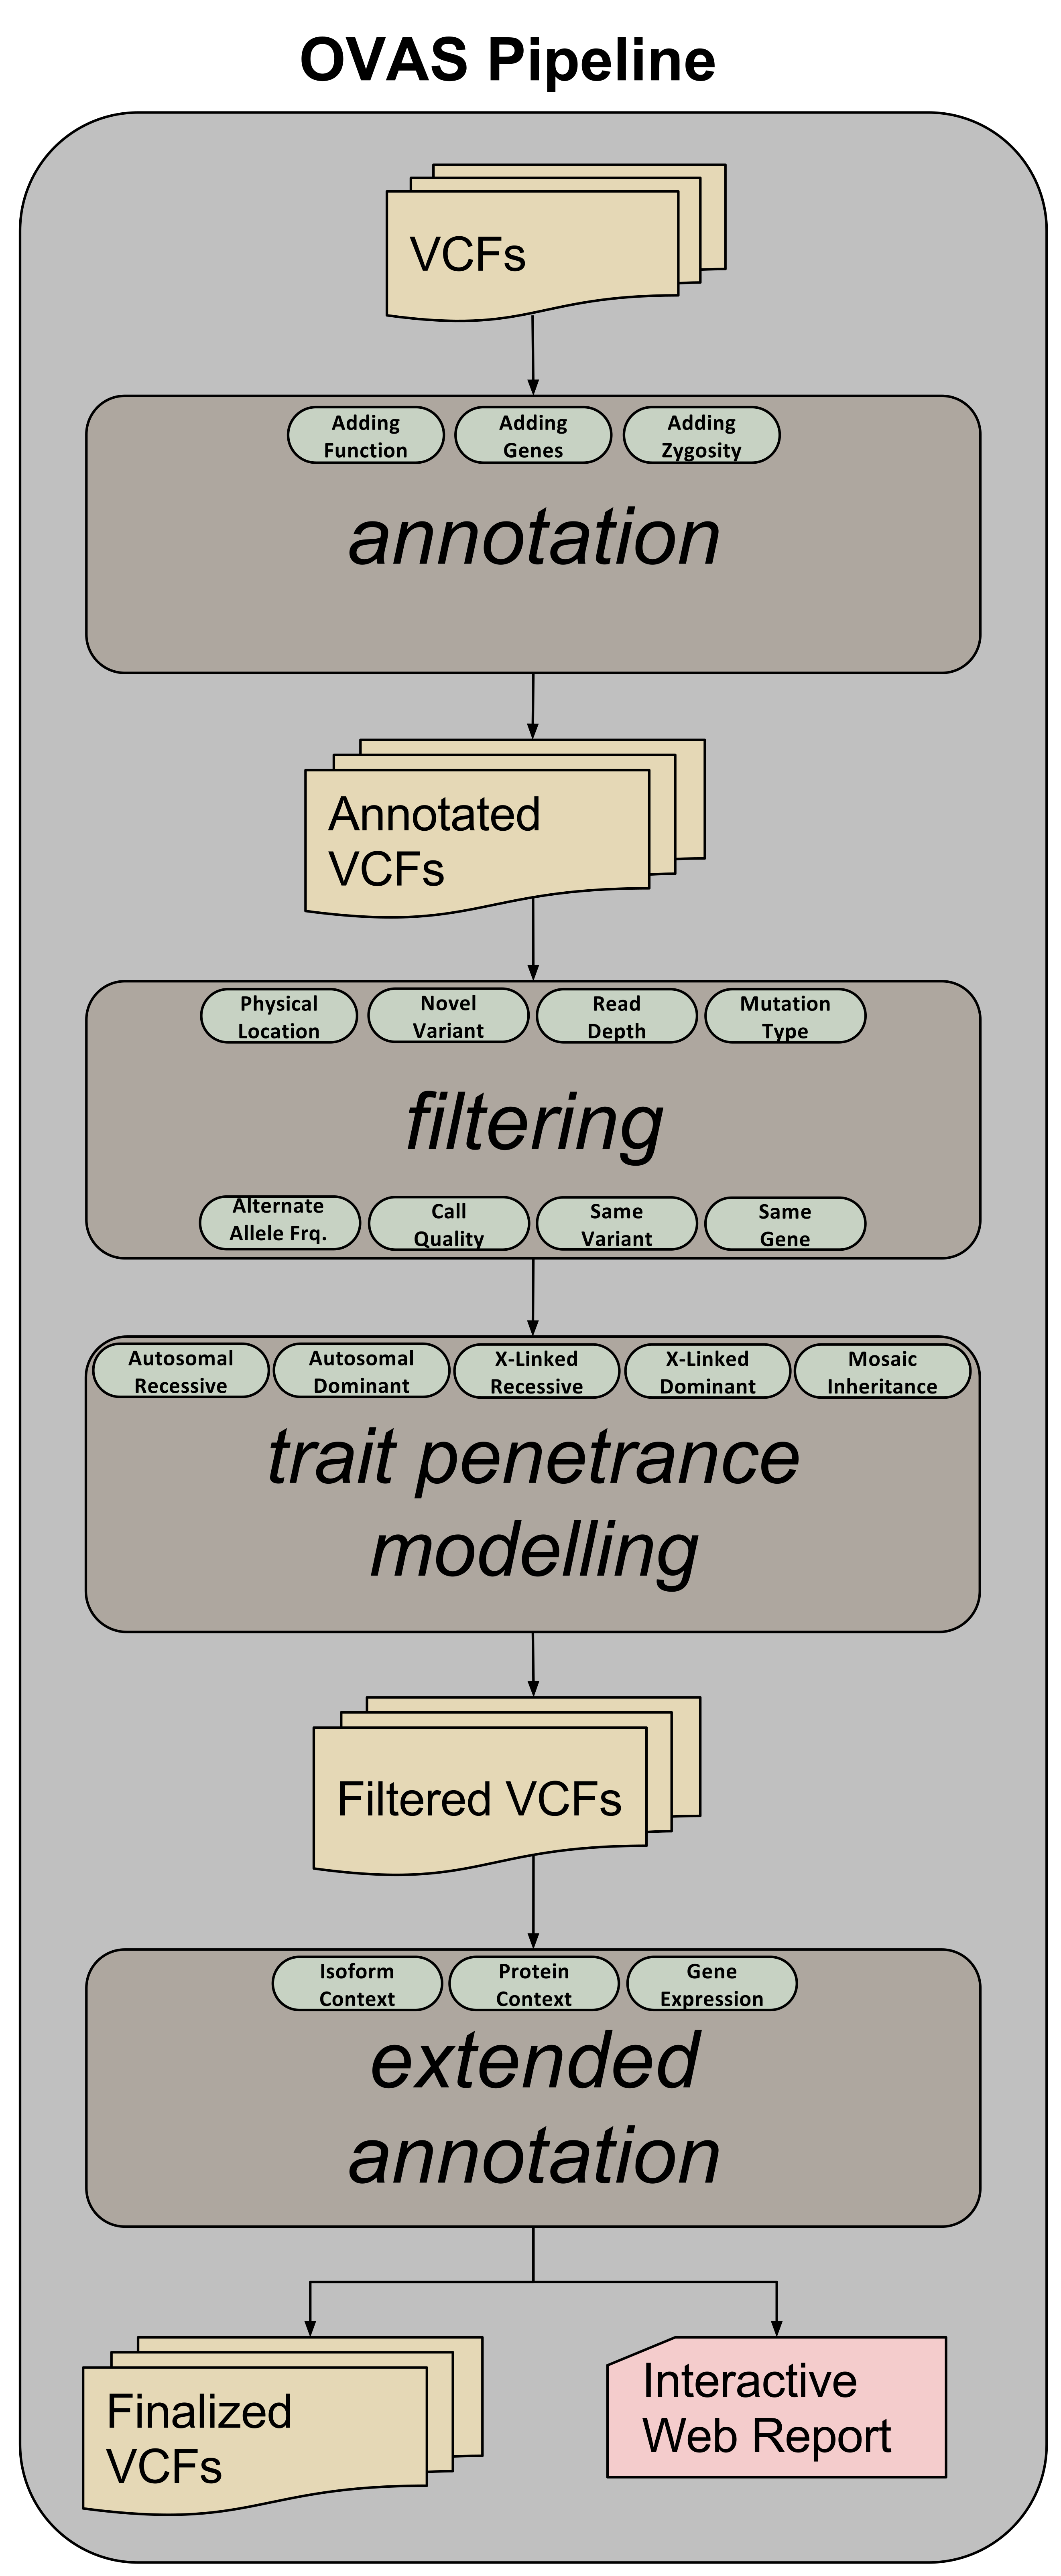
\includegraphics[width=0.45\textwidth]{fig1.png}}
  \caption{\csentence{}Overall structure of the \app{} pipeline: VCF files as referenced by a pedigree file are fed into the pipeline and are processed in turn by the core annotation, optional filtering, trait penetrance modelling, and additional annotation modules. \label{fig1}}
\end{figure}
\begin{figure}[h!]
  %\centerline{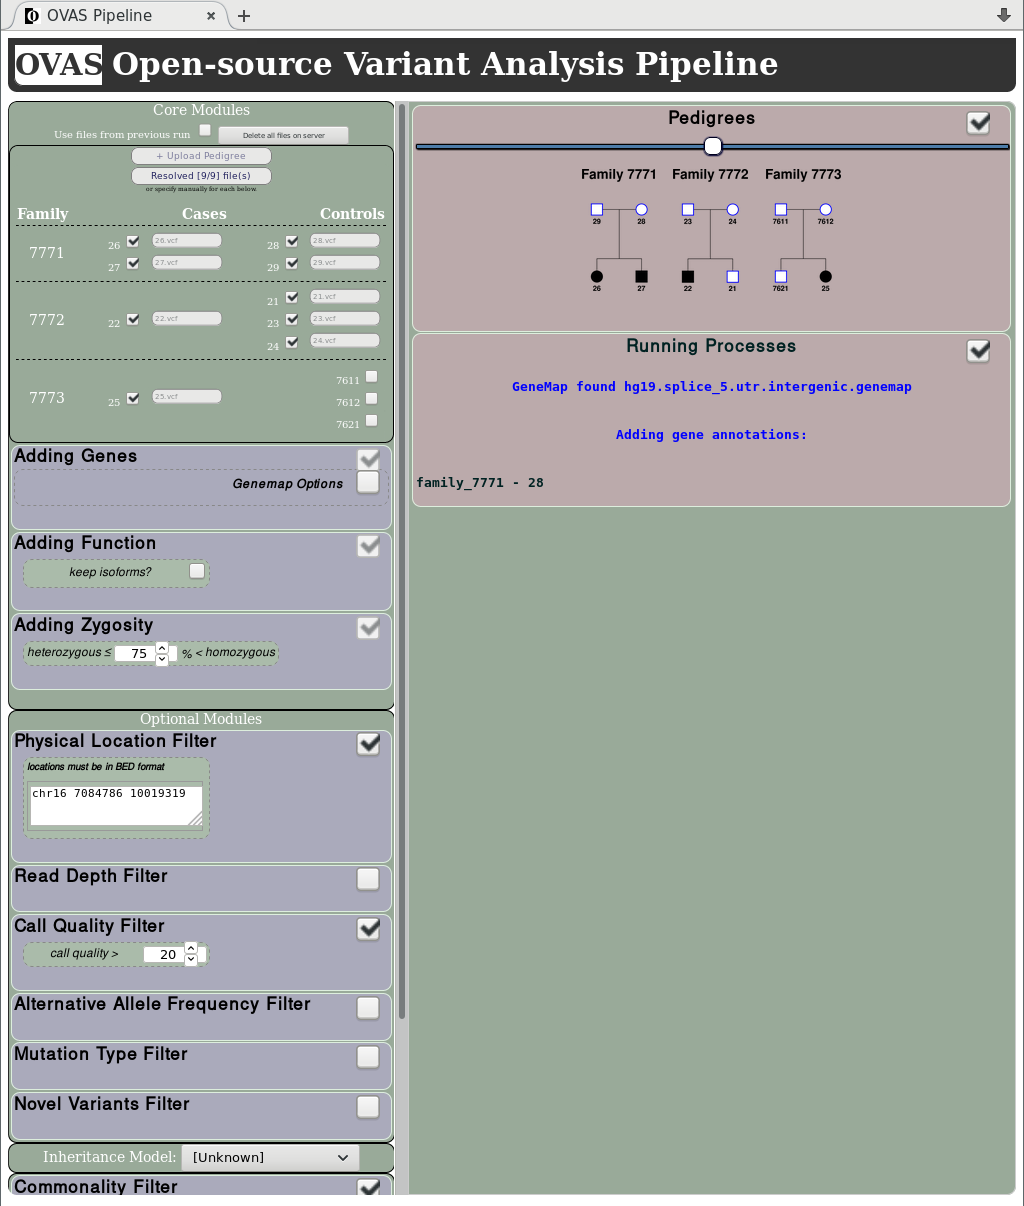
\includegraphics[width=0.45\textwidth]{fig2.png}}
\caption{\csentence{}Web-interface displaying an ongoing analysis. The left sidebar shows the user-set configurations, and the central-right box displays the pedigrees used in the analysis stacked above a real-time progress box. Once complete, a summary will automatically open in a new browser tab. Here, 4 individuals' data from 3 families were analysed, with pipeline settings configured in the left side-bar; case VCF files auto selected, core modules running on default settings, optional modules configured to use linkage data, call quality filtering ($>$20), rare variant filtering ($<1\%$), non-synonymous mutations requested, and an autosomal recessive inheritance filtering model applied in conjunction with gene-level variant filtering.
\label{fig2}}
\end{figure}
\begin{figure}[h!]
  %\centerline{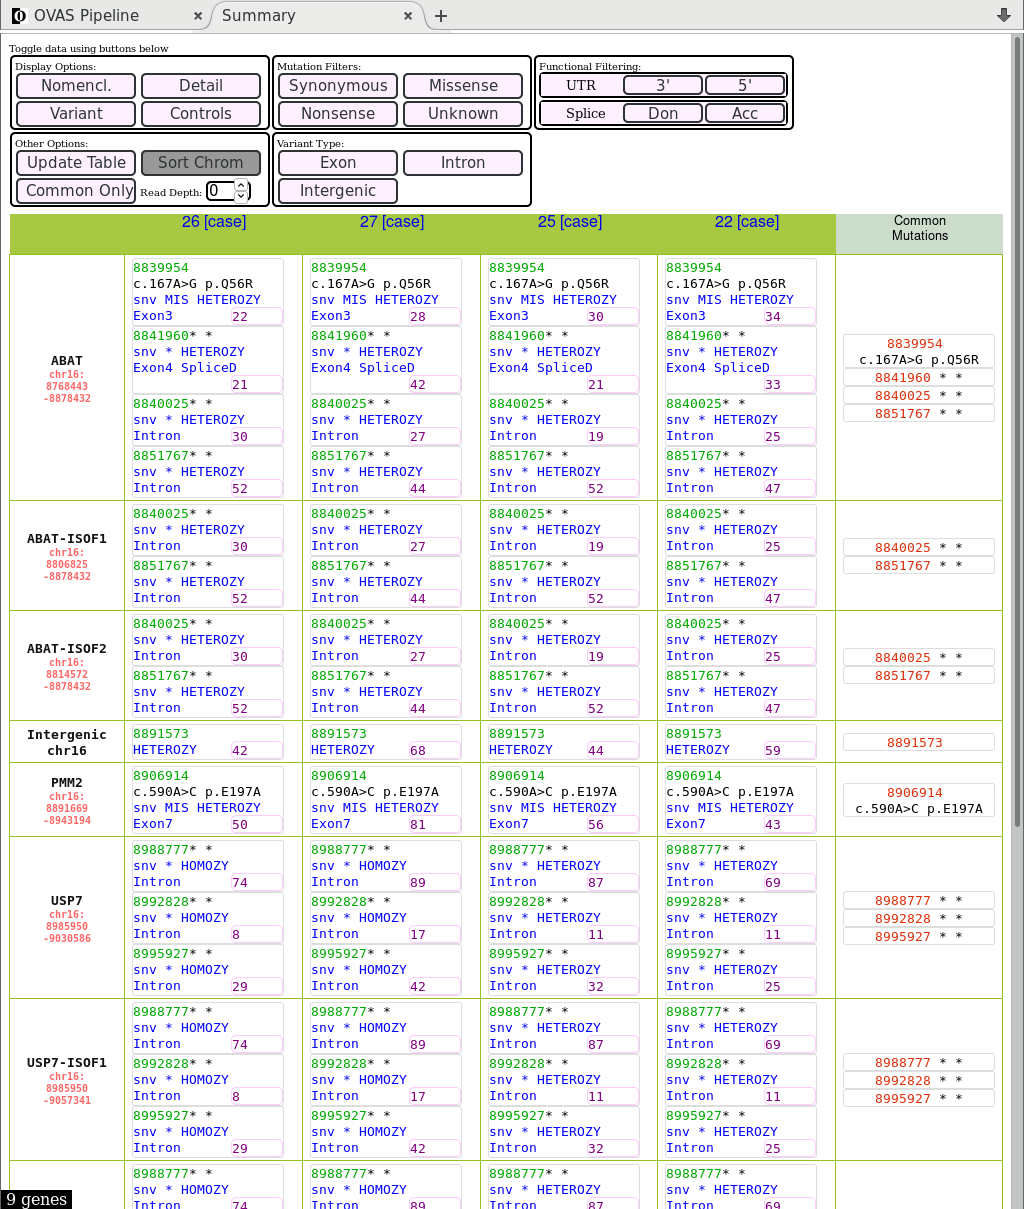
\includegraphics[width=0.45\textwidth]{fig3.png}}
\caption{\csentence{}The summary tab contains a comprehensive report of potential causative variants discovered in the analysis. The report is interactive and can perform dynamic filtering and sorting upon any data field. Columns containing adjacent data in the rows above or below are merged for conciseness. Toggling the column headers sorts the data in that field in ascending/descending order, and the search bar can be used to isolate variants of interest such as those which cause missense mutations, or variants existing in promoter regions. Gene isoforms can be filtered in or out by using the ``ISO'' or ``REF'' keyword, respectively. Pedigrees can be quickly viewed by hovering over the \textit{Show Pedigrees} button above the \textit{Cases} and \textit{Controls} column headers, each of which display the presence and zygosity of the variant in sample individuals, with striped colouring for heterozygous and solid colouring for homozygous. Presented are the same 4 individuals from Figure~\ref{fig2}, showing compound-heterozygous mutations in \textit{PMM2}. Note, the promoter mutation is located within a bidirectional promoter region (i.e. \textit{PMM2/TMEM186}).
\label{fig3}}
\end{figure}
\begin{figure}[h!]
  %\centerline{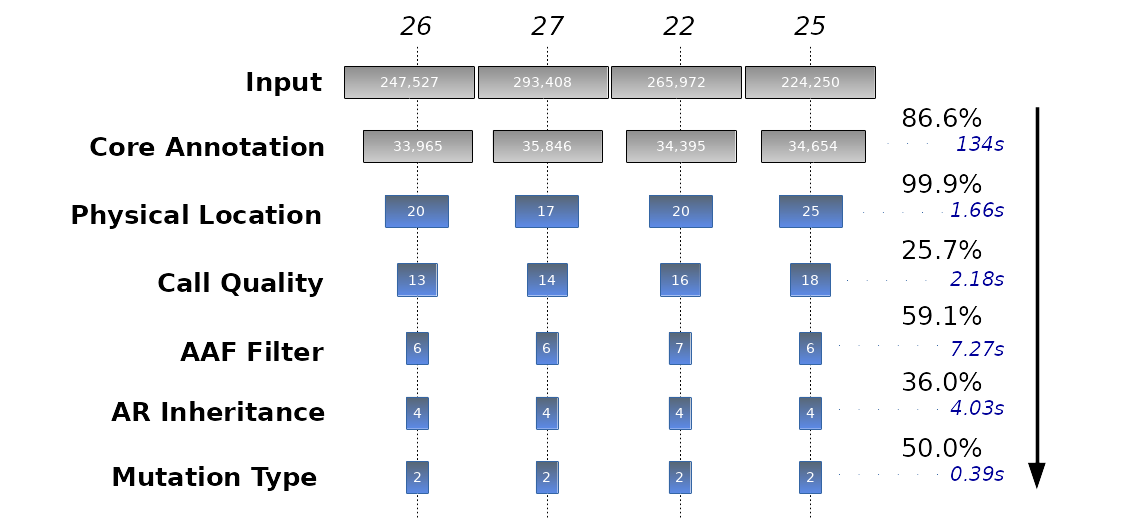
\includegraphics[width=0.45\textwidth]{fig4.png}}
\caption{\csentence{}The progression of variants filtered at each subsequent annotation or filtering stage for each of the 4 case VCFs under initial positional filtering. Input and Core Annotation are mandatory steps. Average variant reduction percentages in-between stages are displayed, and average module runtimes are displayed in seconds.\label{fig4}}
\end{figure}


%%%%%%%%%%%%%%%%%%%%%%%%%%%%%%%%%%%
%%                               %%
%% Tables                        %%
%%                               %%
%%%%%%%%%%%%%%%%%%%%%%%%%%%%%%%%%%%

%% Use of \listoftables is discouraged.
%%
\section*{Tables}

%% Results table
\begin{table}[h!]
\begin{tabular}{| c | *2c |} \hline %\toprule
\emph{Pipeline Stage} & \emph{Module Name} & \emph{Runtime (seconds)} \\
\hline
% A multirow would be more benefial here
% but let's keep package req down for now
             & Adding Genes     & 125\\
Annotation   & Adding Function & 28.7\\
             & Adding Zygosity & 0.81\\
\hline
             & Physical Location Filter & 1.02 \\
             & Read Depth Filter        & 1.26 \\
             & Call Quality Filter      & 0.93\\
Filtering    & AAF Filter               & 143\\
             & Mutation Type Filter     & 1.08\\
             & Novel Variant Filter     & 1.12\\
             & Same Gene Filter       & 22.5\\
             & Same Variant Filter    & 26.1\\
\hline
             & AD Inheritance    & 0.83\\
 Trait       & AR Inheritance    & 1.22\\
Penetrance   & XD Inheritance    & 0.74\\
  Model      & XR Inheritance    & 1.39\\
             & Mosaicism         & 0.94\\
\hline
                 & Isoform Context      & 2.28\\
   Extended      & Protein Context      & 4.10\\
 Annotation      & Gene Expression      & 145\\
\hline
%\botrule
\end{tabular}
\vspace{1ex}
\caption{Average single-core runtimes of VCF files containing 50,000 variants passing individually through all filters with timings for each Annotation, Filtering, and Extended Annotation modules. Trait Penetrance module timings are based on three VCFs consisting of a parent-offspring trio. Tests were run on a 2GHz dual-core processor with 4GB RAM.}\label{table:results}
\end{table}




%%%%%%%%%%%%%%%%%%%%%%%%%%%%%%%%%%%
%%                               %%
%% Additional Files              %%
%%                               %%
%%%%%%%%%%%%%%%%%%%%%%%%%%%%%%%%%%%

\end{backmatter}
\end{document}
